\chapter{Definição do Problema de Estudo}

A estrutura básica de um veículo elétrico é exibida na Figura \ref{fig:estrutura-veiculo-eletrico}. O bloco conversor CA-CC no diagrama representa todo o carregador \textit{onboard} do
 veículo elétrico, incluindo tanto o retificador PFC quanto o conversor CC-CC isolado. O sistema de carregamento pode ser unidireccional ou bidirecional. No primeiro
 caso, o sistema apenas converte a energia da rede elétrica para o veículo, enquanto no segundo caso, o veículo pode fornecer energia de volta para a rede elétrica, o que é conhecido como
\textit{Vehicle-to-Grid} (V2G). O banco de baterias do veículo é composto por células de lítio e ultracapacitores, que são ulizados para armazenar a energia elétrica fornecida pelo carregador.
O inversor é responsável por converter a tensão CC da bateria em uma tensão CA, que aciona o motor do sistema de tração do veículo. Como ilustrado no diagrama, o inversor geralmente é
bidirecional, o que permite o uso de frenagem regenerativa. 

Os carregadores de veículos elétricos são divididos em carregadores \textit{onboard} e \textit{offboard}. Os carregadores \textit{onboard} são instalados dentro do veículo e são 
projetados para serem leves e compactos, devido a restrições de espaço e peso. A potência de saída desses carregadores está na faixa de 0 a 7 kW para sistemas monofásicos e de 0 a 22 kW
para sistemas trifásicos \cite{Yuan:2021}.

\begin{figure}[h]
    \centering
    \caption{Estrutura básica de um veículo elétrico.}
    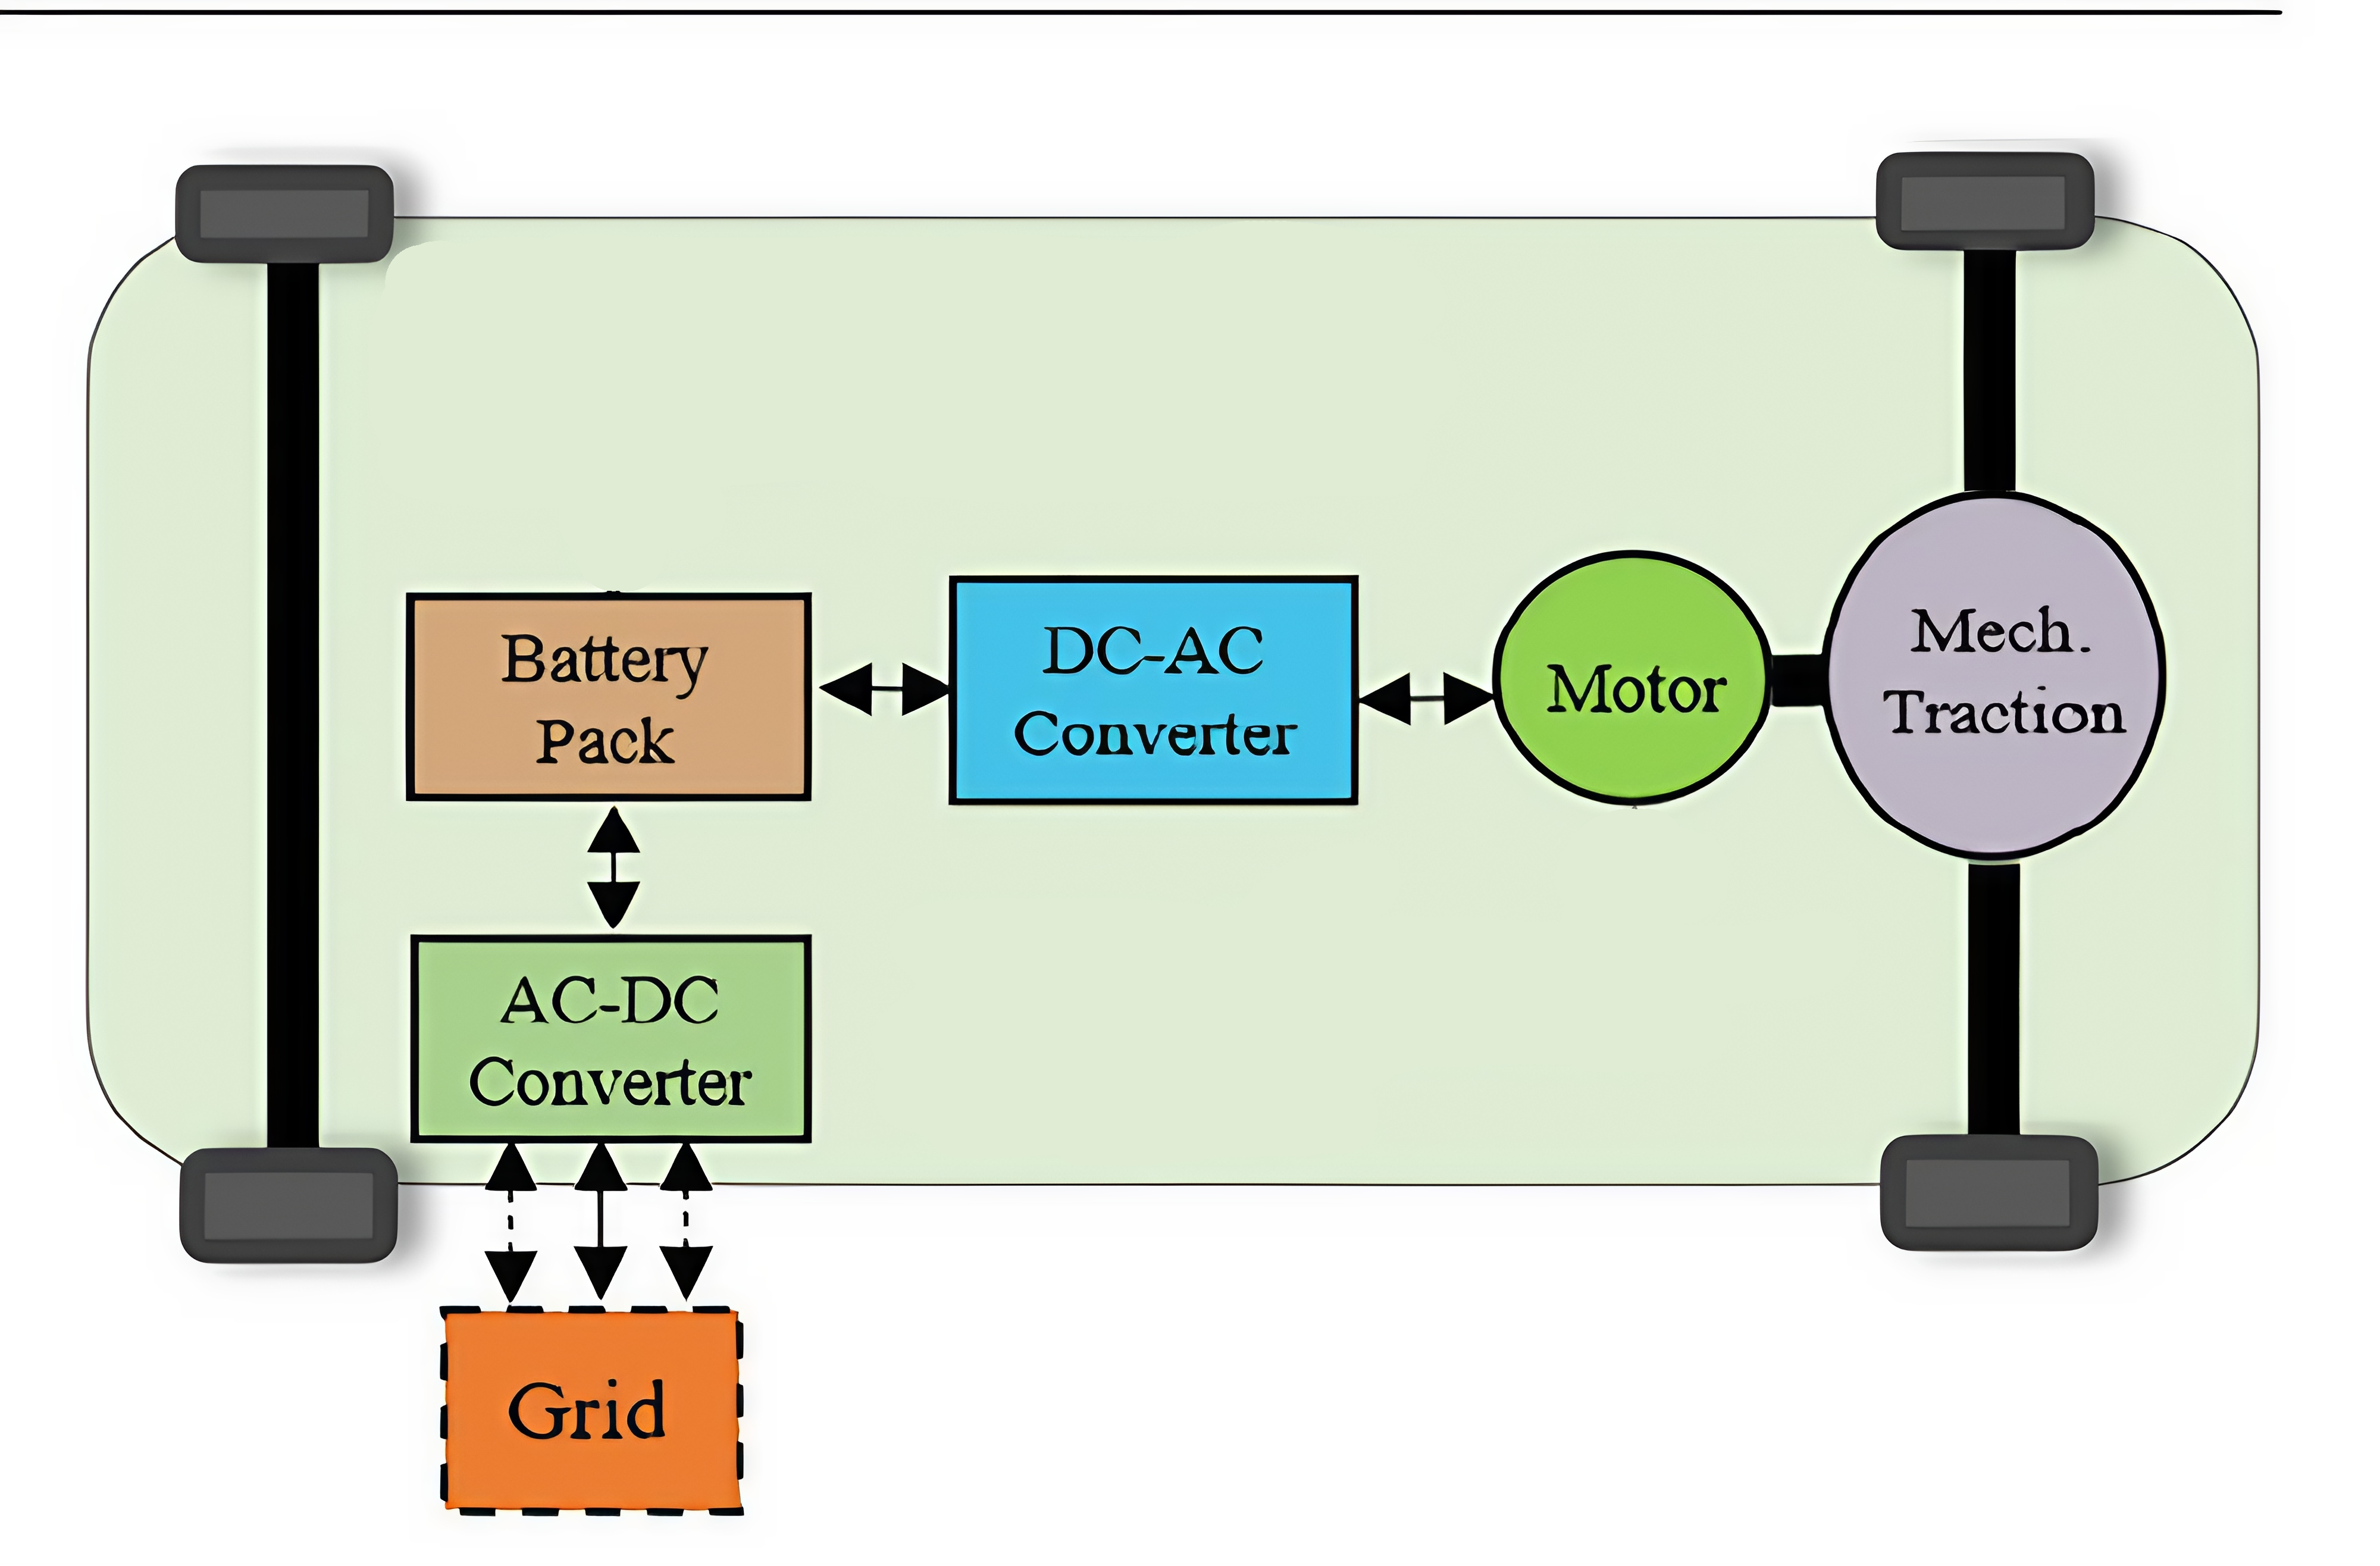
\includegraphics[width=0.8\textwidth]{figuras/diagrama_veiculo_eletrico_edit.png}
    \legend{Fonte: Adaptado de \cite{Kumar:2021}.}
    \label{fig:estrutura-veiculo-eletrico}
\end{figure}

%Falar sobre necessidade de transição energética e adoção de veículos elétricos.

A falta de infraestrutura para o carregamento de veículos elétricos e a preocupação devido a baixa autonomia são citadas em \cite{Karneddi:2021} como
um dos principais gargalos para a adoção em massa desse tipo de veículo. Considerando esses desafios,
o seguinte trabalho propõe o projeto de um carregador \textit{onboard} que seja adequado à realidade do sistema de distribuição
brasileiro. Dessa forma, escolhe-se trabalhar com um sistema de carregamento trifásico.



\section{Objetivo Geral}
O objetivo geral do trabalho é projetar um carregador de veículo elétrico \textit{onboard} trifásico, composto por um retificador PFC e um conversor CC-CC isolado.
\section{Objetivos Específicos}
\begin{itemize}
    \item Realizar revisão bibliográfica sobre as diferentes topologias utilizadas no carregamento de carros elétricos;
    \item Projeto do circuito retificador PFC trifásico;
    \item Sintonia do controlador do retificador PFC trifásico;
    \item Projeto do conversor CC-CC \textit{Phase-Shifted Full Bridge};
    \item Projeto do conversor CC-CC \textit{Dual Active Bridge}(DAB);
    \item Comparação entre o \textit{Phase-Shifted Full Bridge} e o DAB.
\end{itemize}